\section{Theoretical Analysis}
\label{sec:analysis}

In this section, the circuit shown in \textbf{Figure~\ref{fig:diagram_t5}} is analysed
theoretically.
\begin{figure}[h] \centering
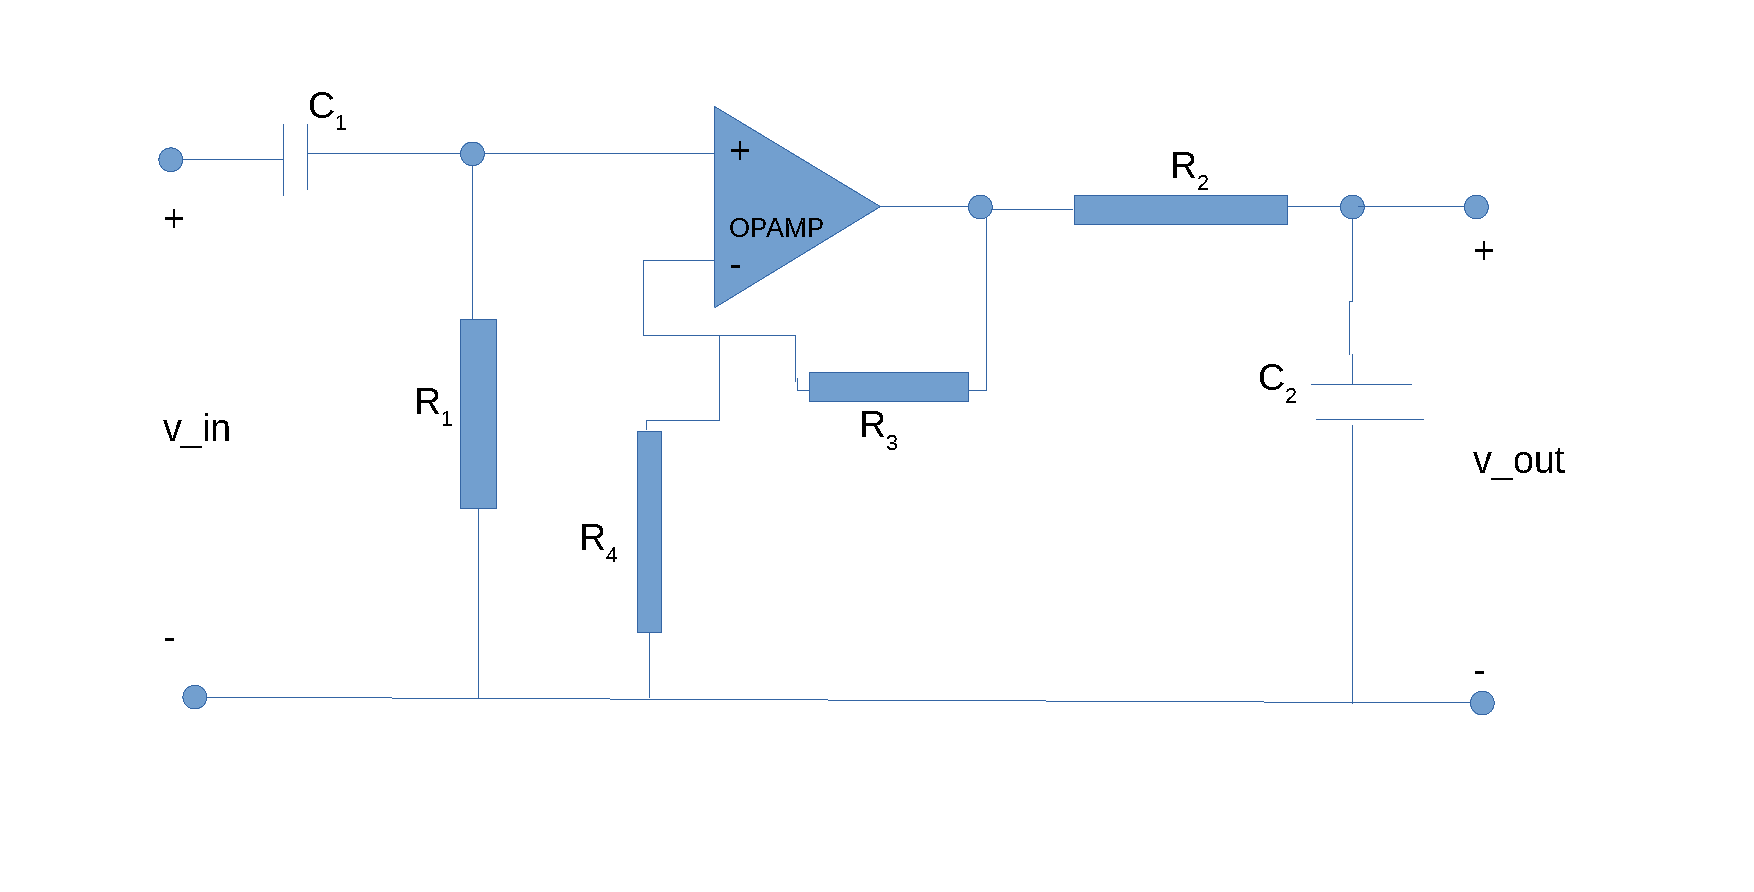
\includegraphics[width=0.95\linewidth]{diagram_t5.pdf}
%\vspace{-7cm}
\caption{Diagram of the circuit considered for the computations and simulations.}
\label{fig:diagram_t5}
\end{figure}


The objective of an OP-AMP Bandpass filter (active bandpass filter) is to, as the name suggests,block unwanted frequencies only allowing a certain bandwith of frequencies to pass through whilst amplifing the signal. In this particular case we want  the central frequency to be 1 KHz and the gain at this frequency to be 40 dB. This filter is a bit different from the one done in a previous lab, that only filter the signal and did not amplified it (passive filter). For  a passive filter we would only need resistors and capacitors, but for an active filter we also need transitors or OP-Amps in order to amplifie the signal. In this case we will use the 741 OP-AMP in an non inverting manner.\par 


The lower cutoff frequency for the circuit shown in \textbf{Figure~\ref{fig:diagram_t5}} will therefore be:
\begin {equation}
	Lower Cutoff Frequency= \frac{1}{R_1*C_1*2*\pi}   
	\label{eq:lcf}
\end{equation}


and the upper cutoff frequency is given by: 

\begin {equation}
	Lower Cutoff Frequency= \frac{1}{R_2 *C_2* 2*\pi}  
	\label{eq:ucf}
\end{equation}

the central frequency is given by:

\begin {equation}
	Central Frequency= \sqrt{Lower Cutoff Frequency * Upper Cutoff Frequency }  
	\label{eq:CentralF}
\end{equation} 
 
the gain is given by:

\begin {equation}
	Gain= \frac{R_1*C_1*W_O*j}{1+R_1*C_1*W_O*j}*(1+\frac{R_3}{R_4})*\frac{1}{1+R_2*C_2*W_O*j}   	
	\label{eq:gain}
\end{equation} 
the transfer function is given by: 

\begin {equation}
	Transfer Function= \frac{R_1*C_1*2*\pi*freq*j}{1+R_1*C_1*2\pi*j}*(1+\frac{R_3}{R_4})*\frac{1}{1+R_2*C_2*2\pi*freq*j}   	
	\label{eq:gain}
\end{equation} 

and the input and output impedances are given by: 

\begin {equation}
	Z_{in} = R_1 + \frac{1}{j*W_O*C_1} 
	\label{eq:impedances_in}
\end{equation}  

\begin {equation}
       Z_{out} = \frac{1}{j*W_O*C_2+\frac{1}{R2}}	
	\label{eq:impedances_out}
\end{equation}  


With materials available  for this lab, and through trial and error whilst having in consideration the formulas above, the final values considered for the circuit parameters (as named in the above figure) that maximized the merit were the following:

%\hfill
% \parbox{1\linewidth}{
%  \centering
%  \begin{tabular}{|l|l|l|r|}
%    \hline    
%    {\bf Parameter} & {\bf Value} & {\bf Units }\\ \hline
%    \input{valores.tex}
%  \label{tab:params}
%  \end{tabular}
%  }
%\par

In the following table the results (output voltage gain in the passband, the central frequency, and the input and output impedances at this frequency) for both for the theoretical analysis (right) and the Ngspice simulation (left) are presented in order to make a side-by-side comparison. \par

%\hfill
% \parbox{1\linewidth}{
%  \centering
%  \begin{tabular}{|l|l|l|r|}
%    \hline    
%    {\bf Node Voltage} & {\bf Simulation} & {\bf Theoretical } & {\bf Units }\\ \hline
%    Vbase & 1.3841 & 1.3841 & V\\ \hline
Vcoll & 8.6547 & 8.6547 & V\\ \hline
Vemit & 0.6855 & 0.6855 & V\\ \hline
Vemit2 & 9.3974 & 9.3974 & V\\ \hline
Vin & 0.0000 & 0.0000 & V\\ \hline
Vin2 & 0.0000 & 0.0000 & V\\ \hline
Vout & 0.0000 & 0.0000 & V\\ \hline
Vvcc & 12.0000 & 12.0000 & V\\ \hline

%  \label{tab:op_FAR}
%  \end{tabular}
%  }
%\par
The circuit used to compute the lower cutoff frequency and the gain, theoretically, was the following incremental model (which includes the coupling capacitors given that these are the limiting factors in terms of the lower cutoff frequency). For the upper cutoff frequency it is a little bit more complex given that this is due to the parasitic capacitances of the transistor, which are part of the Ngspice model, but were not considered in the theory.\par 

%\begin{figure}[h] \centering
%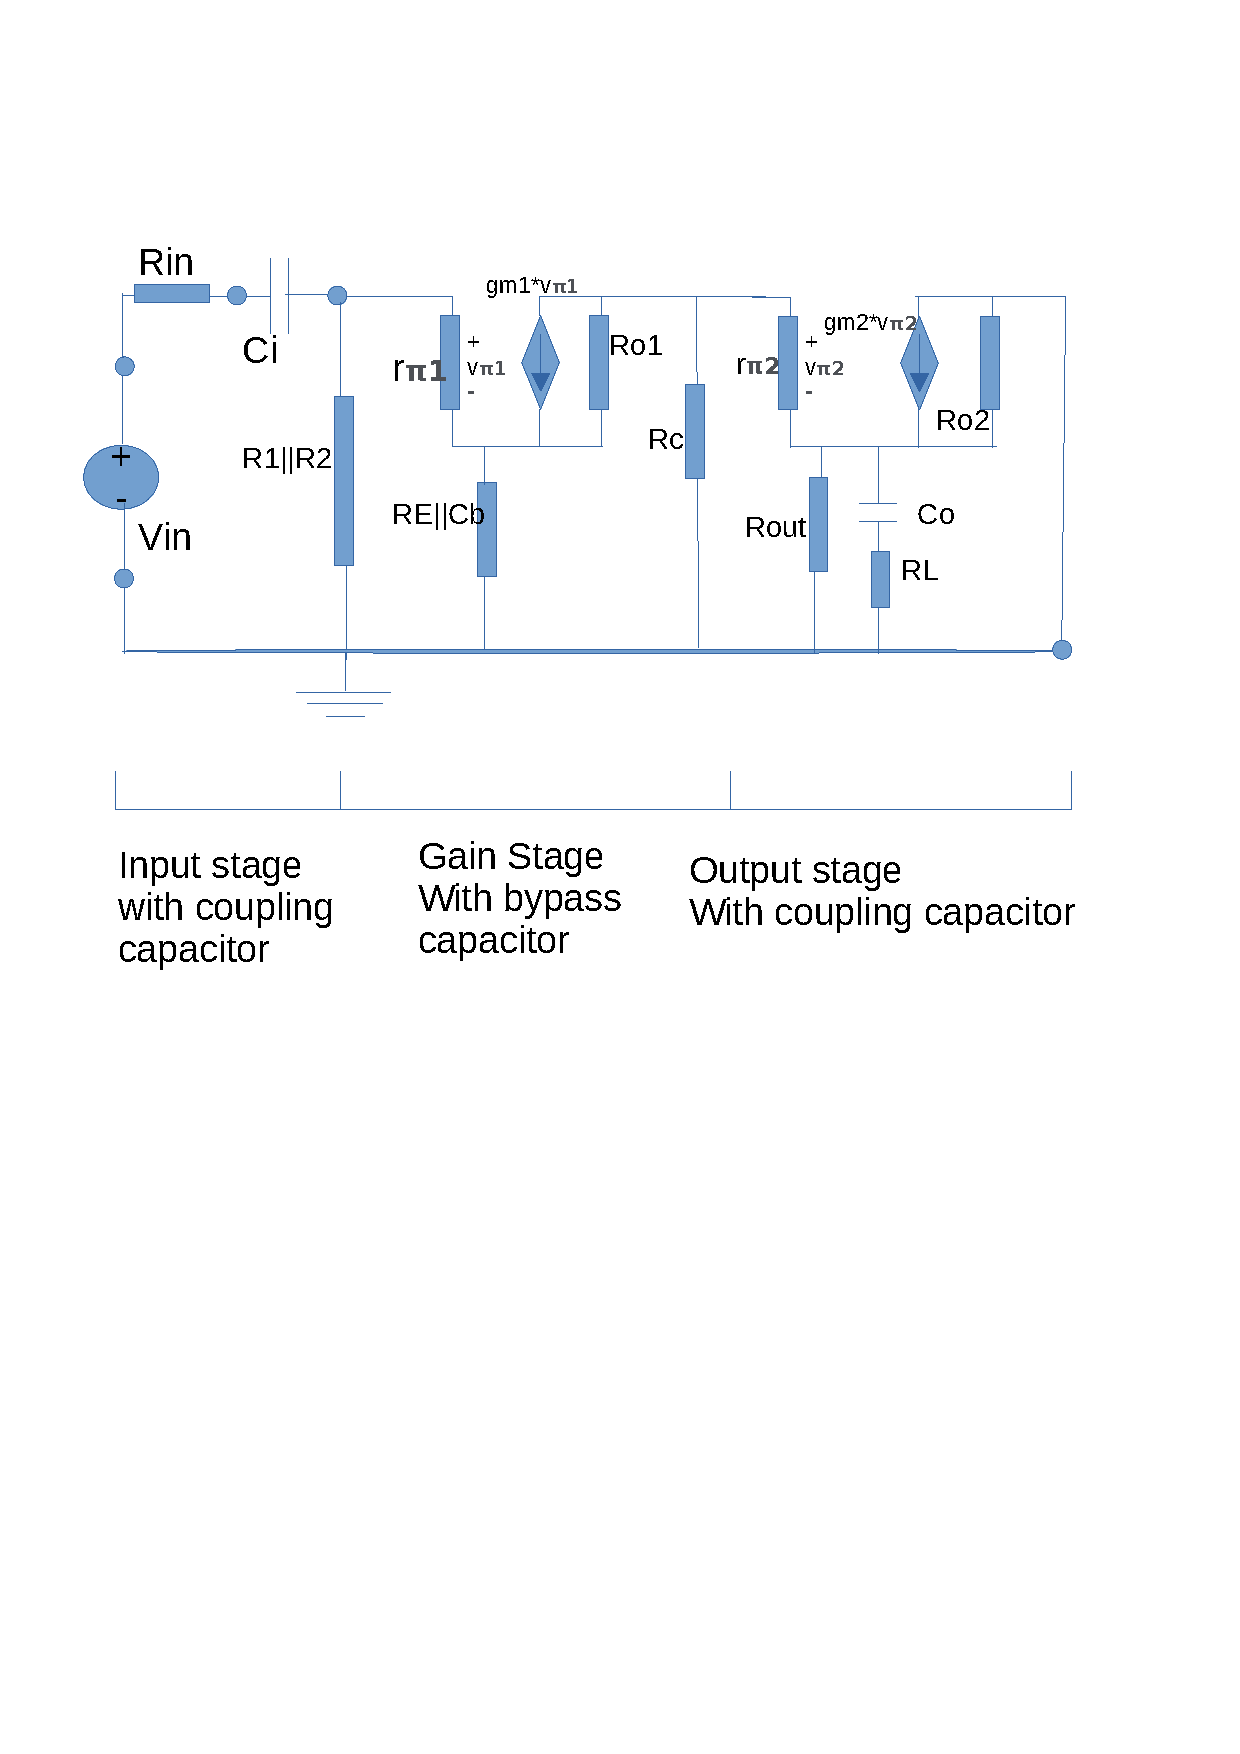
\includegraphics[width=0.95\linewidth]{incremental_t4.pdf}
%\vspace{-7cm}
%\caption{Diagram of the incremental model considered for the gain and frequency response computations.}
%\label{fig:diagram_t4}
%\end{figure}
%\par
%\vspace{1cm}


The gain of the audio amplifier, the upper and lower cut off frequency, the bandwidth and the input and output impedances as well as the merit are presented in the following table, both for the theoretical analysis (right) and the Ngspice simulation (left), in order to make a side-by-side comparison.\par


%\hfill
% \parbox{1\linewidth}{
%  \centering
%  \begin{tabular}{|l|l|l|r|}
%    \hline    
%    {\bf Parameter} & {\bf Simulation} & {\bf Theoretical } & {\bf Units }\\ \hline
%    Zi & 766.402 & 640.49 & Ohm\\ \hline
Zo & 4.49605 & 2.9364 & Ohm\\ \hline
Cost & 8116 & Cost & MU\\ \hline
uco & 3106933.000 & 2123123123123.000 & Hz\\ \hline
lco & 7.924 & 2123123123123.000 & Hz\\ \hline
Bandwidth & 3106925.076 & 2123123123123.000 & Hz\\ \hline
Gainv(out) & 56.041 & -107.220 & [adimensional]\\ \hline
MERIT & 2707.5316 & -104.2260 & gold medals\\ \hline

%  \label{tab:results}
%  \end{tabular}
%  }
  

There was some discrepancy here; for starters note that the input and output impedances for the intermediate stages were not simulated, they were only calculated in theory. The same goes for the gain of the intermediate stages. On a final note, the total input and output impedances of the amplifier were quite different in the two scenarios (theory vs simulation), but of the same order of magnitude; the only other significant difference was the lower cut off frequency.\par

Do note that the upper cutoff frequency here used in the theoretical column was actually obtained from Ngspice: to calculate this frequency in theory, we would need to take into account the parasitic capacitances in the transistor, which proved to be quite more complex and therefore was not used.


  The next figures present the plot of gain obtained in the theoretical analysis.

%In \textbf{Table~\ref{tab:theoretical}} the values for the branch currents and the node voltages obtained from the Octave script for both methods are presented. Here, the node voltages in the mesh method were computed from the respective currents, which were determined as described in the previous subsectio

%\begin{figure}[H] \centering
%\includegraphics[width=0.6\linewidth]{gain_octave.pdf}
%\caption{Output voltage gain of the audio amplifier as a function of frequency}
%\label{fig:gain_octa}
%\end{figure}




\pagebreak


